% 导出独立精修图 PDF（答辩/插图用）
\documentclass[tikz,border=8pt]{standalone}
\usepackage{xeCJK}
\setCJKmainfont{Noto Serif CJK SC}
\usepackage{pgfplots}
\pgfplotsset{compat=1.18,
  every axis/.append style={
    font=\small,
    label style={font=\small},
    tick label style={font=\footnotesize},
    legend style={font=\footnotesize},
    grid=both,
    grid style={line width=.1pt, draw=gray!25},
    major grid style={line width=.2pt,draw=gray!40},
  }
}
\begin{document}

% --- fig-n-latency ---
\begin{tikzpicture}
\begin{axis}[
  width=14cm, height=8cm,
  xlabel={$N$（每 trial 键/文件数）},
  ylabel={PMFS-KV 中位数（$r\_time$）},
  axis y line*=left,
  xmin=4, xmax=36, ymin=0, ymax=45000,
  xtick={8,16,32}, legend pos=north west,
]
\addplot+[thick, mark=*, mark size=2.5pt] coordinates {(8,9206)(16,12168)(32,35830)};
\addlegendentry{PMFS-KV}
\end{axis}
\begin{axis}[
  width=14cm, height=8cm,
  ylabel={xv6 fs+sync 中位数},
  axis y line*=right, axis x line=none,
  xmin=4, xmax=36, ymin=0, ymax=4.0e7, xtick=\empty, legend pos=south east,
]
\addplot+[thick, dashed, mark=square*, mark size=2.2pt, red!70!black]
  coordinates {(8,7408714)(16,16440967)(32,33130730)};
\addlegendentry{xv6 fs+sync}
\end{axis}
\end{tikzpicture}

% --- fig-wa-n ---
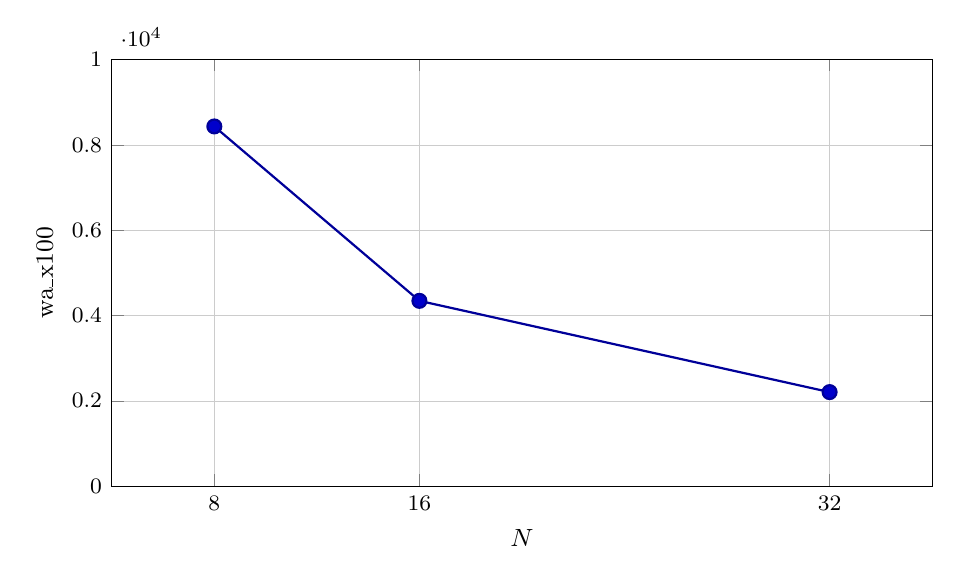
\begin{tikzpicture}
\begin{axis}[
  width=12cm, height=7cm,
  xlabel={$N$}, ylabel={$\mathrm{wa\_x100}$},
  xmin=4, xmax=36, ymin=0, ymax=10000, xtick={8,16,32},
]
\addplot+[thick, mark=*, mark size=2.5pt, blue!60!black]
  coordinates {(8,8432)(16,4344)(32,2205)};
\end{axis}
\end{tikzpicture}

% --- fig-map-emul ---
\begin{tikzpicture}
\begin{axis}[
  ybar, width=10cm, height=7cm,
  ylabel={中位数延迟（$r\_time$）},
  symbolic x coords={EMUL,MAP}, xtick=data,
  ymin=0, ymax=45000, bar width=22pt, nodes near coords,
]
\addplot coordinates {(EMUL,35830)(MAP,26477)};
\end{axis}
\end{tikzpicture}

\end{document}
